
\begin{exercise}
Create a table of values and sketch the graph of the function $y=x^3$ for $-2\leq x\leq 2$. Then use a graphing calculator or other graphing utility to check your graph.
\end{exercise}

\begin{solution}

\begin{minipage}{0.5\textwidth}
\begin{tabular}{|c|c|c|c|c|c|} \hline
$x$ & $-2$ & $-1$ & $0$ & $1$ & $2$ \\ \hline
$y$ & $-8$ & $-1$ & $0$ & $1$ & $8$ \\\hline
\end{tabular}
\end{minipage}
\begin{minipage}{0.5\textwidth}
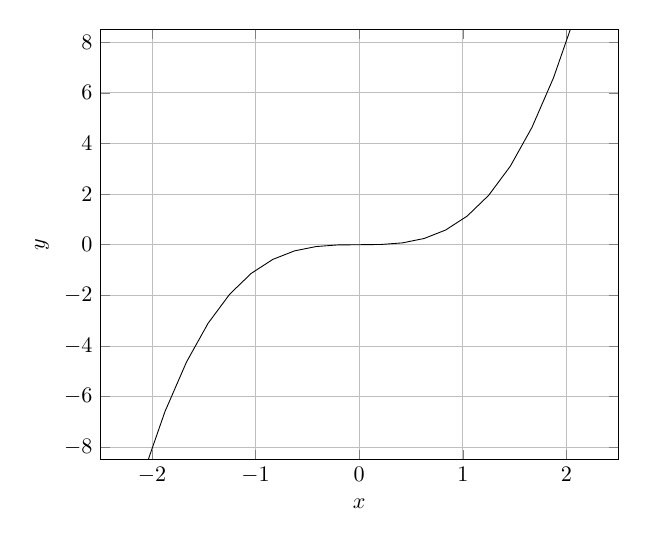
\begin{tikzpicture}[scale=0.8]
\begin{axis}[grid=both,
xmin=-2.5,xmax=2.5,
ymin=-8.5,ymax=8.5,
xtick={-2,-1,...,2},
ytick={-8,-6,...,8},
minor tick={},
xlabel=\(x\), ylabel=\(y\),
x post scale = 1.2,
y post scale = 1.2
]
\addplot[domain=-2.5:2.5] {x^3};
\end{axis}
\end{tikzpicture}
\end{minipage}
\end{solution}





\begin{exercise}
Create a table of values and sketch the graph of the function $f(t)=t^2+t$ for $-2\leq t\leq 1$. Then use your calculator or any other graphing utility to check your graph.
\end{exercise}


\begin{solution}

\begin{minipage}{0.5\textwidth}
\begin{tabular}{|c|c|c|c|c|} \hline
$t$ & $-2$ & $-1$ & $0$ & $1$  \\ \hline
$f(t)$ & $2$ & $0$ & $0$ & $2$ \\\hline
\end{tabular}
\end{minipage}
\begin{minipage}{0.5\textwidth}
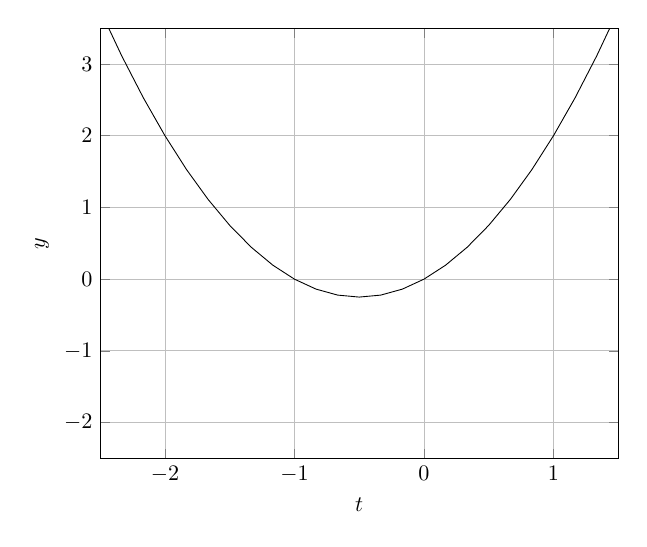
\begin{tikzpicture}[scale=0.8]
\begin{axis}[grid=both,
xmin=-2.5,xmax=1.5,
ymin=-2.5,ymax=3.5,
xtick={-2,-1,...,2},
ytick={-2,...,3},
minor tick={},
xlabel=\(t\), ylabel=\(y\),
x post scale = 1.2,
y post scale = 1.2
]
\addplot[domain=-2.5:1.5] {x^2+x};
\end{axis}
\end{tikzpicture}
\end{minipage}
\end{solution}








\begin{exercise}
Create a table of values and sketch the graph of the function $g(x)=\sqrt{x}$ for $x\geq 0$. Then use a graphing calculator or other graphing utility to check your graph.
\end{exercise}



\begin{solution}

\begin{minipage}{0.5\textwidth}
\begin{tabular}{|c|c|c|c|c|} \hline
$x$ & $0$ & $1$ & $4$ & $9$  \\ \hline
$g(x)$ & $0$ & $1$ & $2$ & $3$ \\\hline
\end{tabular}
\end{minipage}
\begin{minipage}{0.5\textwidth}
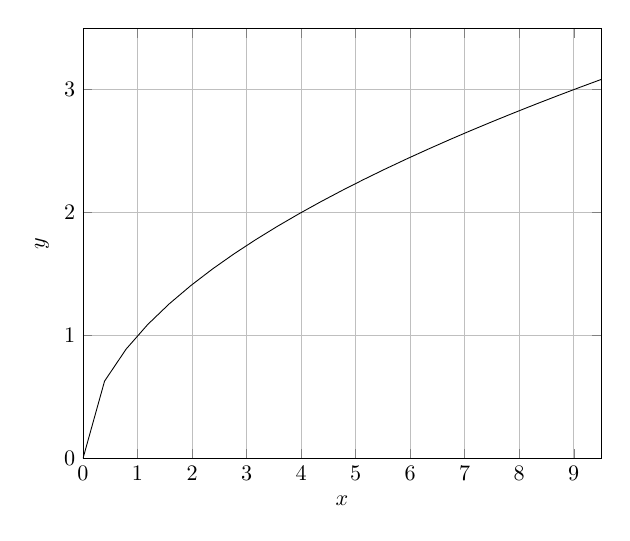
\begin{tikzpicture}[scale=0.8]
\begin{axis}[grid=both,
xmin=0,xmax=9.5,
ymin=0,ymax=3.5,
xtick={0,...,9},
ytick={0,...,3},
minor tick={},
xlabel=\(x\), ylabel=\(y\),
x post scale = 1.2,
y post scale = 1.2
]
\addplot[domain=0:9.5] {x^(1/2)};
\end{axis}
\end{tikzpicture}
\end{minipage}
\end{solution}







\begin{exercise}
The total cost of a meal in a restaurant, $C$, in dollars, as a function of the price of the meal, $p$, in dollars is given by:
\[C=p+0.20p\]
where the term $0.20p$ corresponds to the 20\% tip. Create a table of values and sketch the graph of the function $C=p+0.20p$ for $10\leq p\leq 20$. Then use your calculator or any other graphing utility to check your graph. 
\end{exercise}

\begin{solution}

\begin{minipage}{0.55\textwidth}
\begin{tabular}{|c|c|c|c|c|c|c|}
\hline $p$ & $10$ & $12$ & $14$ & $16$ & $18$ & $20$
\\\hline $C$ & $12$ & $14.4$ & $16.8$ & $19.2$ & $21.6$ & $24$
\\\hline
\end{tabular}
\end{minipage}
\begin{minipage}{0.45\textwidth}
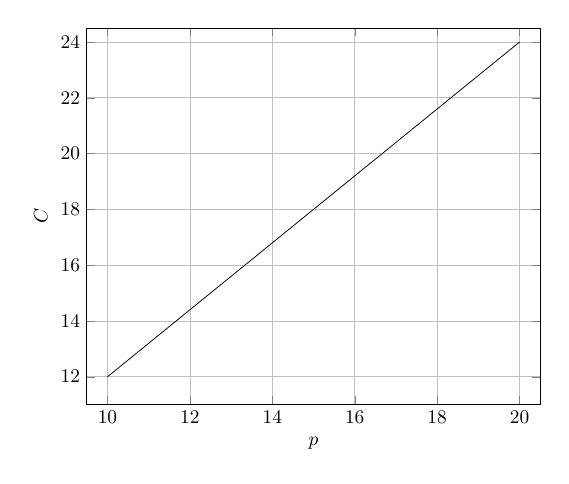
\begin{tikzpicture}[scale=0.7]
\begin{axis}[grid=both,
xmin=9.5,xmax=20.5,
ymin=11,ymax=24.5,
xtick={10,12,14,16,18,20},
ytick={12,14,16,18,20,22,24},
minor tick={},
xlabel=\(p\), ylabel=\(C\),
x post scale = 1.2,
y post scale = 1.2
]
\addplot[domain=10:20] {x+0.2*x};
\end{axis}
\end{tikzpicture}
\end{minipage}
\end{solution}






\begin{exercise}
\label{exercise-1.2-graph1}
Use the graph of the function $y=f(x)$ below to estimate each of the following.



\begin{center}
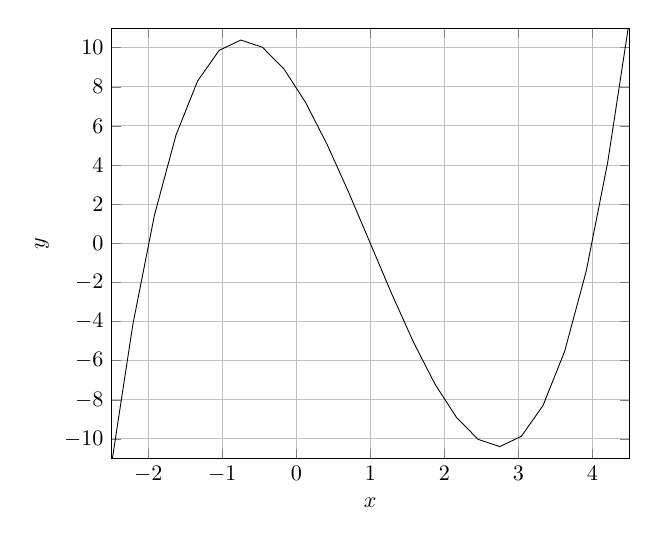
\begin{tikzpicture}[scale=0.8]
\begin{axis}[grid=both,
xmin=-2.5,xmax=4.5,
ymin=-11,ymax=11,
xtick={-2,...,4},
ytick={-10,-8,...,8,10},
minor tick={},
xlabel=\(x\), ylabel=\(y\),
x post scale = 1.2,
y post scale = 1.2
]
\addplot[domain=-2.5:4.5] {(x+2)*(x-1)*(x-4)};
\end{axis}
\end{tikzpicture}
\end{center}


\begin{parts}
\item $f(2)$
\item $f(3)$
\item $f(-1)$
\end{parts}

\end{exercise}



\begin{solution}
\begin{parts}
\item $f(2) = -8$
\item $f(3) = -10$
\item $f(-1) = 10$
\end{parts}
\end{solution}








\begin{exercise}
For the function $y=f(x)$ whose graph is given in Exercise~\ref{exercise-1.2-graph1}, estimate all values $x$ for which $f(x)=0$.
\end{exercise}

\begin{solution}
$x=-2$, $x=1$, and $x=4$.
\end{solution}







\begin{exercise}
For the function $y=f(x)$ whose graph is given in Exercise~\ref{exercise-1.2-graph1}, estimate all values of $x$ for which $f(x)=8$.
\end{exercise}

\begin{solution}
$x\approx -1.5$, $x=0$, and $x\approx 4.5$.
\end{solution}








\begin{exercise}\label{exercise-1.2-graph2}
Use the graph of the function $y = f(t)$ shown below to estimate each of the following.
    \begin{parts}
        \item $f(0)$
        \item $f(12)$
        \item $f(10)$
    \end{parts}
        \begin{center}
        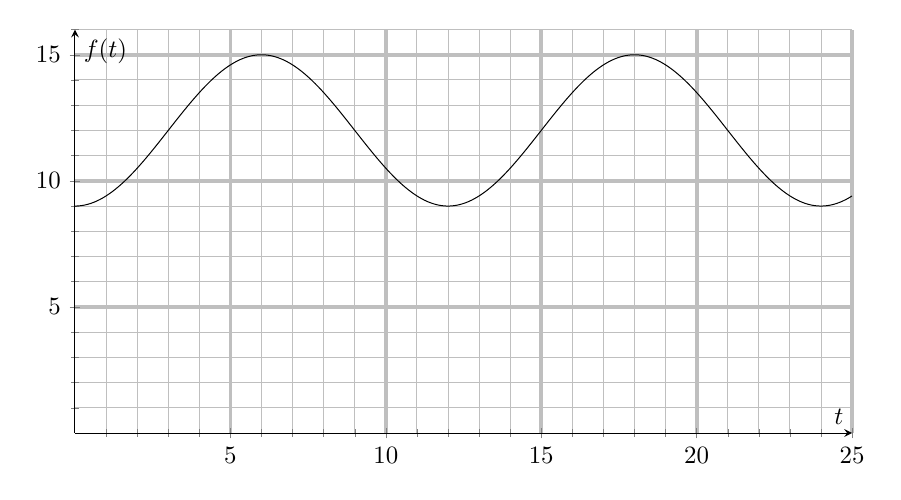
\begin{tikzpicture}[scale=.9]
        \begin{axis}[grid=both,
        axis lines=middle,
        major grid style = {line width = 1.5pt},
        xmin=0,xmax=25,
        ymin=0,ymax=16,
        xtick={5,10,15,20,25},
        ytick={0,5,10,15},
        minor tick={1,...,25},
        xlabel=\(t\), ylabel=\(f(t)\),
        x post scale = 1.6,
        samples=250]
        \addplot[domain=0:25] {-3*cos(deg(3.14159/6*x))+12};
        \end{axis}
        \end{tikzpicture}
        \end{center}

\end{exercise}



\begin{solution}
    \begin{parts}
        \item $f(0)=9$
        \item $f(12)=9$
        \item $f(10)\approx 10.5$
    \end{parts}
\end{solution}







\begin{exercise}
For the function $y = f(t)$ whose graph is given in Exercise~\ref{exercise-1.2-graph2}, estimate all values of $t$ for which $f(t) = 15$.
\end{exercise}



\begin{solution}
$t=6$ and $t=18$
\end{solution}







\begin{exercise}
For the function $y = f(t)$ whose graph is given in Exercise~\ref{exercise-1.2-graph2}, estimate all values of $t$ for which $f(t) = 12$.
\end{exercise}


\begin{solution}
$t=3$, $t=9$, $t=15$, and $t=21$
\end{solution}








\begin{exercise}
A driver of a 2019 Toyota Corolla fills his gas tank and embarks on a highway trip. The amount of gas left in the tank, $G$, in gallons, is a function of the number of miles $m$ driven, $G=g(m)$. Use the graph of $g(m)$ given below to answer the following questions. 


\begin{center}
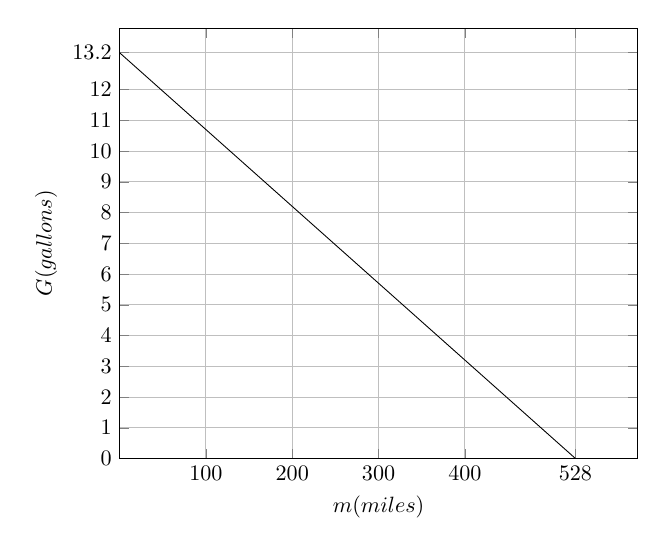
\begin{tikzpicture}[scale=0.8]
\begin{axis}[grid=both,
xmin=0,xmax=600,
ymin=0,ymax=14,
xtick={100,200,300,400,528},
ytick={0,...,12,13.2},
% yticklabels={20,40,60,80,100,120},
minor tick={},
xlabel=\(m\text{ (miles)}\), ylabel=\(G\text{ (gallons)}\),
x post scale = 1.2,
y post scale = 1.2
]
\addplot[domain=0:528] {13.2-(13.2/528)*x};
\end{axis}
\end{tikzpicture}
\end{center}




\begin{parts}
\item What is the fuel tank capacity of the 2019 Toyota Corolla?

\item How much fuel is left after 200 miles?

\item What happens after 528 miles?

\item What is the fuel efficiency of the 2019 Toyota Corolla on the highway?
\end{parts}
\end{exercise}


\begin{solution}
\begin{parts}
\item $13.2$ gallons.
\item $8$ gallons.
\item The gas tank is empty.
\item Approximately $40$ miles per gallon.
\end{parts}
\end{solution}




\begin{exercise}\label{exercise-1.2-caff}
The amount of caffeine remaining in the body, $C$, in milligrams, $t$ hours after drinking a cup of coffee, $C=C(t)$ is given by the graph below.



\begin{center}
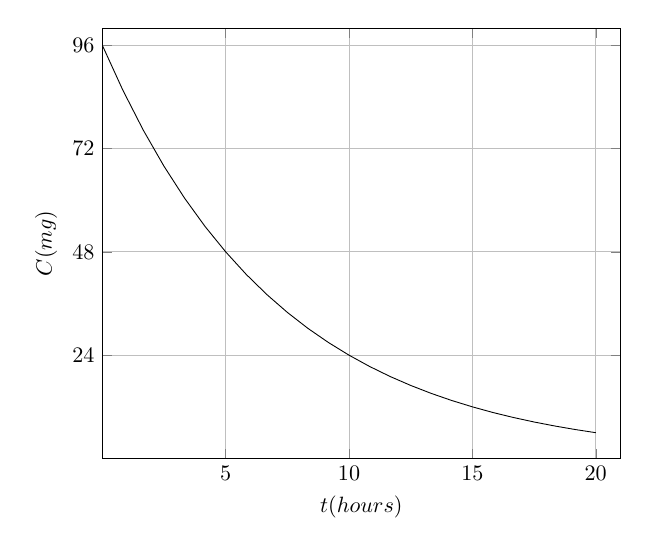
\begin{tikzpicture}[scale=0.8]
\begin{axis}[grid=both,
xmin=0,xmax=21,
ymin=0,ymax=100,
xtick={5,10,...,20},
ytick={24,48,...,96},
minor tick={},
xlabel=\(t\text{ (hours)}\), ylabel=\(C\text{ (mg)}\),
x post scale = 1.2,
y post scale = 1.2
]
\addplot[domain=0:20] {96*(1/2)^(x/5)};
\end{axis}
\end{tikzpicture}
\end{center}




\begin{parts}
\item How much caffeine was absorbed into the bloodstream from the cup of coffee?

\item How much caffeine is left after 5 hours? After 10 hours?

\item Is the function $C(t)$ increasing, decreasing or neither on the interval $t\geq 0$?
\end{parts}
\end{exercise}


\begin{solution}
\begin{parts}
\item $96$ mg.
\item After $5$ hours, there are $48$ mg left. After $10$ hours, $24$ mg.
\item Decreasing.
\end{parts}
\end{solution}


\begin{exercise}
A man deposited money into a savings account. His balance $B(t)$, in dollars, after $t$ years is given by the graph below.


\begin{center}
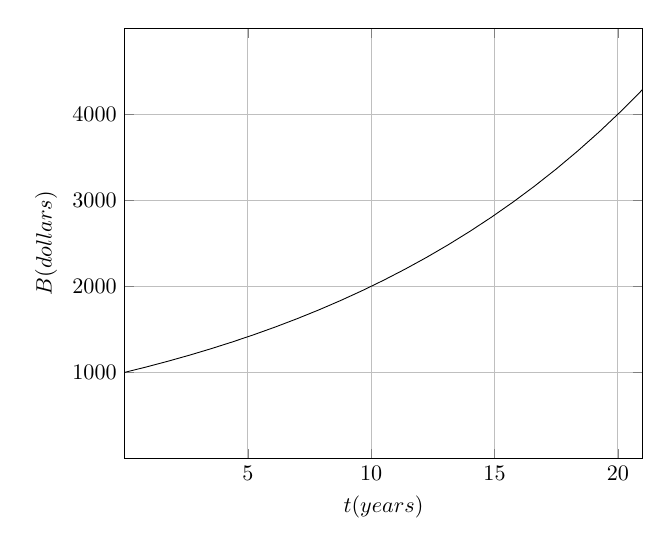
\begin{tikzpicture}[scale=0.8]
\begin{axis}[grid=both,
xmin=0,xmax=21,
ymin=0,ymax=5,
xtick={5,10,...,20},
ytick={1,2,3,4},
yticklabels={1000,2000,3000,4000},
minor tick={},
xlabel=\(t\text{ (years)}\), ylabel=\(B\text{ (dollars)}\),
x post scale = 1.2,
y post scale = 1.2
]
\addplot[domain=0:21] {1*(2)^(x/10)};
\end{axis}
\end{tikzpicture}
\end{center}


\begin{parts}
\item What was his initial deposit?

\item How much money was in his account after 10 years? After 20 years?

\item Is the function $B(t)$ increasing, decreasing or neither in the interval $t\geq 0$?
\end{parts}

\end{exercise}

\begin{solution}
\begin{parts}
\item $\$1000$.
\item After 10 years, $\$2000$. After 20 years, $\$4000$.
\item Increasing.
\end{parts}
\end{solution}



\begin{exercise}
Is the curve below the graph of a function $y=f(x)$? Explain your answer.




\begin{center}
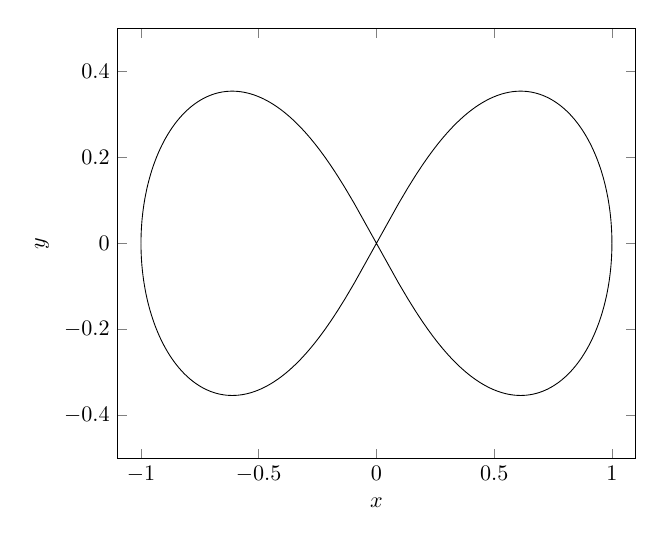
\begin{tikzpicture}[scale=0.8]
\begin{axis}[
xmin=-1.1,xmax=1.1,
ymin=-0.5,ymax=0.5,
xtick={-1,-0.5,...,1},
ytick={-0.4,-0.2,...,0.4},
minor tick={},
xlabel=\(x\), ylabel=\(y\),
x post scale = 1.2,
y post scale = 1.2
]
\addplot [data cs=polar,domain=0:180,samples=361] (\x,{sqrt(cos(2*x))});
\addplot [data cs=polar,domain=0:180,samples=361] (\x,{-sqrt(cos(2*x))});
\end{axis}
\end{tikzpicture}
\end{center}
\end{exercise}


\begin{solution}
No, because it fails the vertical line test (in many places!).
\end{solution}



\begin{exercise}
The graph of a function $y=f(x)$ is given below. Use it to find the following.


\begin{center}
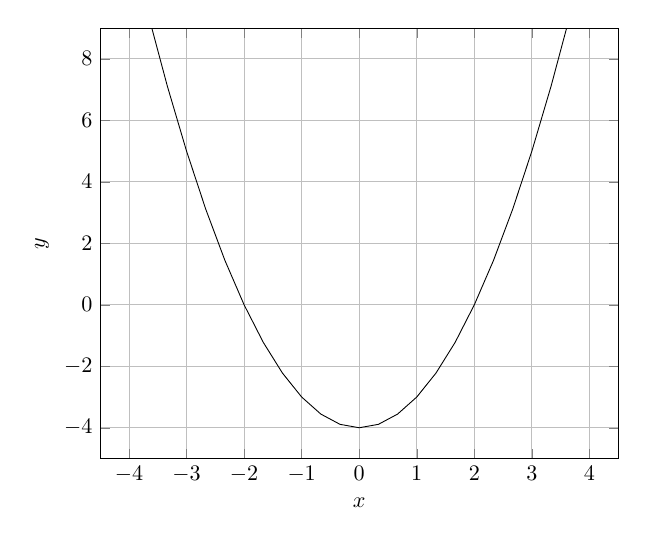
\begin{tikzpicture}[scale=0.8]
\begin{axis}[grid=both,
xmin=-4.5,xmax=4.5,
ymin=-5,ymax=9,
xtick={-4,...,4},
ytick={-4,-2,...,8},
minor tick={},
xlabel=\(x\), ylabel=\(y\),
x post scale = 1.2,
y post scale = 1.2
]
\addplot[domain=-4:4] {x^2-4};
\end{axis}
\end{tikzpicture}
\end{center}


\begin{parts}
\item Estimate $f(0)$.

\item Estimate all values of $x$ for which $f(x)=0$.

\item Estimate all values of $x$ for which $f(x)=5$.
\end{parts}
\end{exercise}

\begin{solution}
\begin{parts}
\item $f(0) = -4$.
\item $x=-2$ and $x=2$.
\item $x=-3$ and $x = 3$.
\end{parts}
\end{solution}



\begin{exercise}
For the function $y=f(t)$ whose graph is depicted below, identify the intervals on the $t$-axis for which the function is increasing and for which the function is decreasing.


\begin{center}
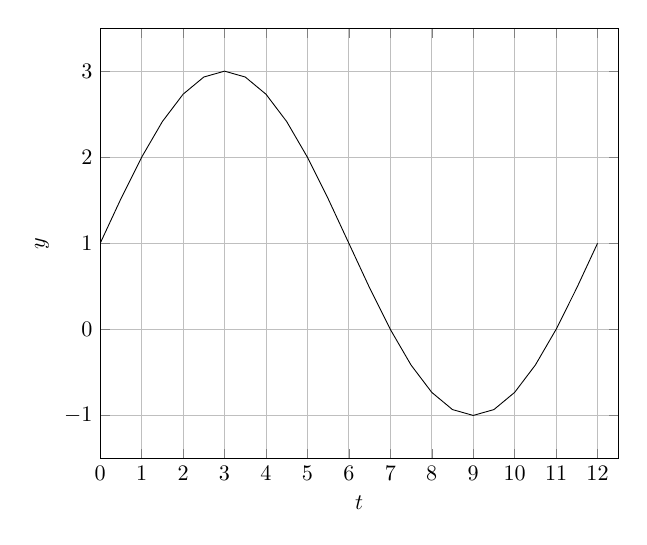
\begin{tikzpicture}[scale=0.8]
\begin{axis}[grid=both,
xmin=0,xmax=12.5,
ymin=-1.5,ymax=3.5,
xtick={0,...,12},
ytick={-1,...,3},
minor tick={},
xlabel=\(t\), ylabel=\(y\),
x post scale = 1.2,
y post scale = 1.2
]
\addplot[domain=0:12] {2*sin(deg(2*pi/12 *x))+1};
\end{axis}
\end{tikzpicture}
\end{center}

\end{exercise}

\begin{solution}
Increasing on the intervals $(0,3) \cup (9,12)$. {\it Or, write as $0<t<3$ and $9<t<12$}.
Decreasing on the interval $(3,9)$. {\it Or, write as $3<t<9$}.
\end{solution}